\documentclass{report}
\usepackage[utf8]{inputenc} % Codificación UTF-8 para caracteres latinos
\usepackage[T1]{fontenc} % Codificación de la fuente para caracteres acentuados
\usepackage[spanish]{babel} % Idioma español
\usepackage{xcolor}
\usepackage{tikz}
\usepackage{graphicx}
\usepackage{pagecolor} % Paquete para cambiar el color de fondo de la página
\usepackage{enumitem}
\usepackage{tabularx}


% Configurar la numeración de subsecciones
\setcounter{secnumdepth}{4}

% Definir un nuevo color personalizado
\definecolor{azulportada}{RGB}{0,25,51} % Color azul RGB

% Paquetes básicos
\usepackage{amsmath} % Paquete matemático
\usepackage{amsfonts} % Fuentes matemáticas
\usepackage{amssymb} % Símbolos matemáticos
\usepackage{graphicx} % Inclusión de gráficos
\usepackage{float} % Control de posición de figuras y tablas
\usepackage{hyperref} % Enlaces hipertexto
\usepackage{geometry} % Configuración de márgenes y tamaño del papel


% Definir información de la portada
\title{Título del Documento}
\author{Jonnathan Torres Vázquez}
\date{\today}

% Configuración de márgenes
\geometry{a4paper, margin=1in}

\begin{document}

\pagecolor{azulportada}
\begin{titlepage}
    \begin{tikzpicture}[remember picture, overlay]
        \node[anchor=north west, inner sep=10pt] at (current page.north west) {
\includegraphics[width=1.5cm]{ICONO2i.png}};
    \end{tikzpicture}

    \vfill
    \begin{center}
        % Título
        \vspace{5cm}
        {\Huge \textbf{Memoria De Cálculo Estructural Para El Proyecto 'Casa Cojitambo'} \par}

        \vspace{15cm}
        {\Large MAMPRO SAS - Abril 2024 \par}
        
    \end{center}
    \vfill
\end{titlepage}

% Restablecer el color de fondo a blanco
\pagecolor{white}

\chapter{Introducción}
El presente proyecto estructural tiene como objetivo el diseño y análisis de una casa de un piso ubicada en la parroquia Cojitambo, en el cantón Azogues, Ecuador. Esta región, caracterizada por su belleza natural y su contexto geográfico particular, presenta desafíos específicos en términos de diseño y construcción para garantizar la seguridad y estabilidad de las estructuras ante las condiciones locales.

La casa de un piso se diseñará cumpliendo con las normativas y regulaciones de construcción ecuatorianas vigentes, garantizando la resistencia sísmica adecuada y considerando las cargas gravitacionales y de viento pertinentes para esta ubicación geográfica. Además, se utilizará el software ETABS en conjunto con Python, aprovechando su potencial para la modelización, análisis y optimización de estructuras, así como su capacidad para interactuar con la API de ETABS.

El desarrollo de este proyecto implica una cuidadosa planificación y un análisis detallado, con el fin de asegurar la integridad estructural y la durabilidad de la vivienda, proporcionando un entorno seguro y confortable para sus futuros ocupantes.

\section{Objetivos}
\begin{enumerate}[label = \alph*]
    \item Diseñar una estructura residencial segura y funcional que cumpla con las normativas y regulaciones de construcción ecuatorianas aplicables, garantizando la seguridad de los ocupantes.
    \item Optimizar el diseño estructural para maximizar la eficiencia en el uso de materiales y recursos, asegurando un balance adecuado entre costo, resistencia y durabilidad.
    \item Integrar consideraciones sísmicas específicas para la región de Cojitambo, utilizando técnicas de análisis avanzadas para evaluar y mitigar los efectos de los movimientos telúricos en la estructura.
    \item Implementar prácticas sostenibles de construcción que minimicen el impacto ambiental del proyecto, incluyendo la selección de materiales ecoamigables y soluciones de diseño que fomenten la eficiencia energética.
    \item Utilizar herramientas computacionales como el software ETABS y Python para modelar, analizar y optimizar la estructura, aprovechando las ventajas de la tecnología para mejorar la precisión y la eficacia del proceso de diseño.
    \item Colaborar estrechamente con otros profesionales involucrados en el proyecto, como arquitectos, ingenieros civiles y contratistas, para garantizar la coherencia y la integración de los aspectos estructurales con el diseño arquitectónico y los requisitos de construcción.
    \item Proporcionar documentación detallada y clara, incluyendo planos, cálculos y especificaciones técnicas, que sirva como guía para la construcción y el mantenimiento de la estructura a lo largo de su vida útil.
\end{enumerate}

\section{Normativa y Regulaciones Aplicables}
\begin{enumerate}
    \item  Diseñar una estructura residencial segura y funcional que cumpla con las normativas y regulaciones de construcción ecuatorianas aplicables, garantizando la seguridad de los ocupantes.

    \item Optimizar el diseño estructural para maximizar la eficiencia en el uso de materiales y recursos, asegurando un balance adecuado entre costo, resistencia y durabilidad.

    \item Integrar consideraciones sísmicas específicas para la región de Cojitambo, utilizando técnicas de análisis avanzadas para evaluar y mitigar los efectos de los movimientos telúricos en la estructura.

    \item Implementar prácticas sostenibles de construcción que minimicen el impacto ambiental del proyecto, incluyendo la selección de materiales ecoamigables y soluciones de diseño que fomenten la eficiencia energética.

    \item Utilizar herramientas computacionales como el software ETABS y Python para modelar, analizar y optimizar la estructura, aprovechando las ventajas de la tecnología para mejorar la precisión y la eficacia del proceso de diseño.

    \item Colaborar estrechamente con otros profesionales involucrados en el proyecto, como arquitectos, ingenieros civiles y contratistas, para garantizar la coherencia y la integración de los aspectos estructurales con el diseño arquitectónico y los requisitos de construcción.

    \item Proporcionar documentación detallada y clara, incluyendo planos, cálculos y especificaciones técnicas, que sirva como guía para la construcción y el mantenimiento de la estructura a lo largo de su vida útil.
\end{enumerate}

Por supuesto, es importante mencionar que además de la Norma Ecuatoriana de la Construcción NEC-15, se emplearán normativas internacionales reconocidas como la ACI 19 (American Concrete Institute) y la AISC (American Institute of Steel Construction), que proporcionan estándares y criterios ampliamente aceptados en la industria de la construcción. Algunos puntos a destacar sobre la utilización de estas normativas son:
\begin{enumerate}
    \item  \textbf{ACI (American Concrete Institute)}: Se utilizarán las especificaciones y criterios de diseño de la ACI 19 para el diseño de elementos de concreto, como columnas, vigas, losas y cimentaciones. 
    
    La ACI  proporciona recomendaciones detalladas sobre la resistencia del concreto, la disposición de refuerzos, los factores de seguridad y otros aspectos relevantes para garantizar la seguridad y durabilidad de las estructuras de concreto.
    
    \item \textbf{AISC (American Institute of Steel Construction)}: Se seguirán las normativas y estándares de la AISC para el diseño de elementos estructurales de acero, incluyendo vigas, columnas, conexiones y sistemas de arriostramiento.
    
    La AISC establece criterios para la selección de perfiles estructurales, el diseño de conexiones soldadas y atornilladas, así como otros aspectos relacionados con la resistencia y estabilidad de las estructuras de acero.
    Al integrar normativas como la ACI 19 y la AISC en el proceso de diseño y cálculo estructural, se garantiza que la estructura cumpla con estándares de calidad y seguridad reconocidos a nivel internacional, además de los requisitos locales establecidos por la Norma Ecuatoriana de la Construcción NEC-15. Esta combinación de normativas permite obtener diseños estructurales robustos y confiables que se adecuan a las condiciones y exigencias específicas del proyecto en Cojitambo, Azogues.
\end{enumerate}

\section{Descripción del diseño estructural}
faltaaaaaaaaaaaaaaaaa

\chapter{Cargas y Combinaciones}
La NEC15 establece que en general las contrucciones deberán diseñarse para resistir las 
combinaciones de cargas permanentes, cargas variables y cargas accideantales.

%INICIA SECCION CARGAS, OBTENIDO CON FUNCIONES DE PYTHON

\section{Cargas Permanentes}
Las cargas permanentes consideradas para el proyecto son:
\begin{enumerate}
    \item[\textbullet] Fibrocemento = 0.16 $KN/m^2$
    \item[\textbullet] Acero en fr\'io = 0.08 $KN/m^2$
    \item[\textbullet] Acero en caliente = 1.2 $KN/m^2$
    \item[\textbullet] Instalaciones = 1 $KN/m^2$
    \item[\textbullet] Cielo Raso = 0.5 $KN/m^2$
    
\end{enumerate}
\section{Cargas Variables}
Para el proyecto unicamente existen sobrecargas variables de cubierta. La NEC se\~{n}nala que
la carga de cubierta es de 0.7

\section{Cargas de granizo}
Seg\'un la NEC se debe considerar una acumulaci\'on de granizo en un corto periodo de tiempo.
Para cubiertas con pendientes menores de 15\% se debe considerar una carga m\'inima de 0.50 $kN/m^2$; 
para cubiertas con pendientes menores del 5\% se debe considerar 1.0 kN/m2. Se determinan de la siguiente forma:

$$S = \rho H_s$$

Donde:

$\rho $: Peso espec\'ifico del granizo (en defecto: 1000 $Kg/m^3$)

$H_s$: Altura de acumulaci\'on ($m$)
\\
La f\'ormula mencionada nos da una carga de granizo igual a 2.0

\section{Cargas Por viento}
Para obtener las cargas por viento primero hay que calcular la velocidad del viento. Para esto la 
NEC nos da la siguiente f\'ormula: 
$$V_b = V \cdot \alpha$$

Donde:

$V_b$: Velocidad corregida del viento en $m/s$

$V$: Velocidad instant\'anea m\'axima del viento en m/s, registrada a 10 m de altura sobre el terreno.

\begin{table}[h]
    \centering
    \begin{tabular}{|c|c|c|}
        \hline
        Coef. de correlaci\'on&Velocidad instant\'anea&Velocidad corregida\\
        &(m/s)&(m/s)\\
        \hline
        0.91&&19.11\\
        \hline
    \end{tabular}
\end{table}

\subsection{Presi\'on del viento}
La NEC establece la siguiente f\'ormula para el c\'alculo de la presi\'on del viento:
$$P = \frac{1}{2} \rho V_b^2 c_e c_f$$

Donde:

$P$: Presi\'on de c\'alculo expresada en Pa $N/m^2$

$\rho$: Densidad del aire expresada en $Kg/m^3$ (En general, se puede adoptar 1.25 $Kg/m^3$)

$c_e$ : Coeficiente de entorno/altura

$c_f$ : Coeficiente de forma
\\
Con la f\'ormula se obtienen los valores del Barlovento y Sotavento, cuyos valores son presentados
en las siguientes tablas.

    \begin{table}[h]
        \centering
        \resizebox{\textwidth}{!}{
            \begin{tabular}{|c|c|c|c|c|}
                \hline
                Densidad del aire ($kg/m^3$) & Velocidad del viento ($m/s$) & Coef. Entorno/altura & Coef. De forma & Barlovento ($kN/m^2$)\\
                \hline
                1.25&19.11&0.3&0.8&0.054778815\\
                \hline
            \end{tabular}
            }
    \end{table}
    
    \begin{table}[h]
        \centering
        \resizebox{\textwidth}{!}{
            \begin{tabular}{|c|c|c|c|c|}
                \hline
                Densidad del aire ($kg/m^3$) & Velocidad del viento ($m/s$) & Coef. Entorno/altura & Coef. De forma & Barlovento ($kN/m^2$)\\
                \hline
                1.25&19.11&-0.6&0.8&-0.10955763\\
                \hline
            \end{tabular}
            }
    \end{table}
        
\section{Cargas de granizo}
Seg\'un la NEC se debe considerar una acumulaci\'on de granizo en un corto periodo de tiempo.
Para cubiertas con pendientes menores de 15\% se debe considerar una carga m\'inima de 0.50 $kN/m^2$; 
para cubiertas con pendientes menores del 5\% se debe considerar 1.0 kN/m2. Se determinan de la siguiente forma:
    
$$S = \rho H_s$$

Donde:

$\rho $: Peso espec\'ifico del granizo (en defecto: 1000 $Kg/m^3$)

$H_s$: Altura de acumulaci\'on ($m$)
\\
La f\'ormula mencionada nos da una carga de granizo igual a 2.0

\section{Carga s\'ismica}
Para obtener el valor de la carga s\'ismico se construye el espectro a partir de los datos de la geolog\'ia local determinados
por el estudios de suelos.
De esta manera los pa\'arametros que permiten la construcci\'on del espectro de acuerdo a la NEC son:

\begin{enumerate}
    \item[\textbullet] \textbf{Fa} - Coeficiente de amplificaci\'on de suelo en la zona de periodo corto.
    \item[\textbullet] \textbf{Fd} - Desplazmiento para dise\~no en roca.
    \item[\textbullet] \textbf{Z} - Factor de zona s\'simica.
    \item[\textbullet] \textbf{n} - Raz\'on entre la aceleraci\'on espectral Sa (T = 0.1 s) y el PGA para el periodo de retorno seleccionado.
    \item[\textbullet] \textbf{r} - Factor usado en el espectro de dise\~no el\'astico, cuyos valores dependen de la ubicaci\'on geogr\'afica del proyecto.
\end{enumerate}

Los valores de los par\'ametros se muestran en la siguiente tabla:

    \begin{table}[h]
        \centering
            \begin{tabular}{|c|c|c|c|c|c|c|c|}
                \hline
                \textbf{ZONA SISMICA} & \textbf{Perfil suelo} & \textbf{Fa} & \textbf{Fd} & \textbf{Fs} & \textbf{Z} & \textbf{r} & \textbf{n}\\
                \hline
                0.25 & E & 1.5 & 1.75 & 1.6 & 0.25 & 1.5 & 2.48\\
                \hline
            \end{tabular}
    \end{table}
    
    Con los valores presentados en la tabla se grafica el espectro.
    
    \begin{figure}[h]
        \centering
        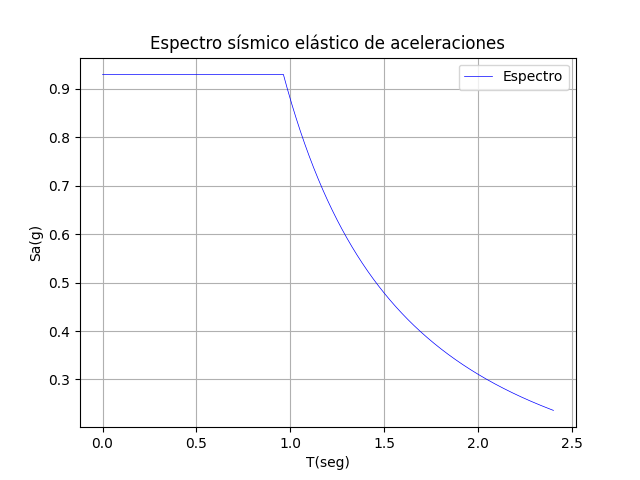
\includegraphics[width=0.5\textwidth]{imagenes/espectro.png}
    \end{figure}
%%%%%%%%%%%%%%%

\section{Combinaciones para el dise\~no de \'ultima resistencia}
La NEC se\~nala que las estructuras, componentes y cimentaciones deber'an dise\~narse
para que la resistencia de dise\~no iguale o supere las siguientes combinaciones:

\begin{enumerate}
    \item \textbf{Combinaci\'on 1} - 1.4D
    \item \textbf{Combinaci\'on 2} - 1.2D + 1.6L+ 0.5max(Lr ; S ; R)
    \item \textbf{Combinaci\'on 3} - 1.2D + 1.6max(Lr ; S ; R)+ max(L ; 0.5W)
    \item \textbf{Combinaci\'on 4} - 1.2D + 1.0W + L + 0.5 max(Lr ; S ; R)
    \item \textbf{Combinaci\'on 5} - 1.2D + 1.0E + L + 0.2S
    \item \textbf{Combinaci\'on 6} - 0.9D + 1.0W
    \item \textbf{Combinaci\'on 7} - 0.9D + 1.0E
\end{enumerate}

En donde cada s\'imbolo significa:

\begin{enumerate}
    \item[\textbullet] \textbf{D} - Carga permanente
    \item[\textbullet] \textbf{E} - Carga de sismo
    \item[\textbullet] \textbf{L} - Sobrecarga (carga viva)
    \item[\textbullet] \textbf{Lr} - Sobrecarga cubierta (carga viva)
    \item[\textbullet] \textbf{S} - Carga de granizo
    \item[\textbullet] \textbf{W} - Carga de viento
\end{enumerate}

Las cargas para el proyecto se presentan en la siguiente tabla:

\begin{table}[h]
    \centering
    \begin{tabular}{|c|c|c|c|c|}
        \hline
        \textbf{Carga Muerta} & \textbf{Sobrecarga Cubierta} & \textbf{Barlovento} & \textbf{Sotavento} & \textbf{Granizo} \\
        \hline
        2.94 & 0.7 & 0.054 & -0.109 & 2.0\\
        \hline
    \end{tabular}
\end{table}

Las cargas s\'ismcas se calcular\'an con ayuda del programa ETABS.
El proyecto por sus carater\'isticas arquitect\'onicas no cuenta con cargas vivas.

%%%%%%%%%%%%%%

\chapter{Metodolog\'a de dise\~{n}o estructural - Dise\~{n}o basado en fuerzas}
La NEC establece que las estrucuturas deben dise\~{n}arse para resistir fuerzas s\'ismicas provenientes de las 
combinaciones de las fuerzas horizontales. Adem\'as que las fuerzas s\'ismicas de dise\~{n}o act\'uan de manera
no concurrente en la direcci\'on de cada eje principal de la estrucutura para luego ser combinadas de acuerdo a 
las siguientes combinaciones:
\begin{enumerate}
    \item \textbf{Combinaci\'on 1} $E_{h1} = max[(E_x + 0.3E_y), (E_y + 0.3E_x)]$
    \item \textbf{Combinaci\'on 2} $E_{h2} =\pm \sqrt{E_x^2 + E_y^2}$
\end{enumerate}

Donde:

\begin{enumerate}
    \item[\textbullet] $E_{h}$ Componente horizontal de la fuerza s\-ismica
    \item[\textbullet] $E_x$ Componente horizontal de la fuerza s\-ismica seg\'un el eje x
    \item[\textbullet] $E_y$ Componente horizontal de la fuerza s\-ismica seg\'un el eje y
\end{enumerate}

El dise\~{n}ador considerar\'a el siguiente valor de la componente s\-ismica horizontal: 
\begin{enumerate}
    \item \textbf{Combinaci\'on m\'as desfavorable} $E_h = max[E_{h1}, E_{h2}]$
\end{enumerate}
%%%%%%%

\section{Factor de reducci\'on de respuesta R}
La NEC nos indica que el valor del factor de reducci\'on debe ser escogido de acuerdo a criterios relacionados con aspectos de agrupamiento de 
estructuraci\'on, diferencias entre realidades constructivas y de calidad entre los materiales y la construcci\'on, penalizaciones dirigidas hacia cierto tipo de estructuras 
que no permiten 
disponer de ductilidad global apropiada para soportar las deformaciones inel\'asticas requeridas por el sismo de dise\~{n}o. As\'i
tambi\'en depende del tipo de suelo, periodo de vibraci\'on considerado, factores de ductilidad, sobre resistencia, 
redundancia y amortiguamiento de una estructura en condiciones l\'imite.

Inicialmente el valor de R se escoge de la tabla 11 de la NEC-SE-DS, para posteriormente reducirlo de acuerdo a las irregularidades
presentes en la estructura.

\section{Irregularidades estructurales}
Las irregularidades estructurales son desviaciones o caracter\'isticas no deseables en la geometr\'ia, la distribuci\'on 
de masa o la rigidez de un edificio o estructura que pueden afectar su comportamiento s\'ismico y su capacidad para resistir fuerzas laterales, como las producidas por un terremoto. Estas irregularidades pueden influir en la distribuci\'on de las fuerzas y las deformaciones dentro de la estructura 
durante un evento s\'ismico, lo que a su vez puede afectar la seguridad y la estabilidad del edificio. Se clasifiacan en dos tipos,
irregularidades en planta, irregularidades en elevaci\'on.

\subsection{Irregularidades en planta}
\subsubsection{Irregularidad Torsional }
Existe irregularidad por torsi\'on, cuando la m\'axima deriva de piso de un extremo de la estructura calculada incluyendo la torsi\'on accidental y medida perpendicularmente a un eje determinado, es mayor que 1,2 veces la 
deriva promedio de los extremos de la estructura con respecto al mismo eje de referencia.
$$\vartriangle = 1.2 \cdot \dfrac{\vartriangle 1 + \vartriangle 2}{2}$$

\begin{figure}[h]
    \centering
    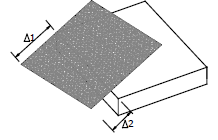
\includegraphics[width=0.15\textwidth]{imagenes/irregularidad_torsional.png}
\end{figure}

\subsubsection{Retrocesos excesivos en las esquinas }
La configuraci\'on de una estructura se considera irregular cuando presenta entrantes excesivos en sus esquinas. 
Un entrante en una esquina se considera excesivo cuando las proyecciones de la estructura, a ambos lados del entrante, 
son mayores que el 15\% de la dimensi\'on de la planta de la estructura en la direcci\'on del entrante.
$$A > 0.15B y C > 0.15D$$

\begin{figure}[h]
    \centering
    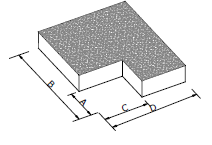
\includegraphics[width=0.15\textwidth]{imagenes/retrocesos_excesivos_en_las_esquinas.png}
\end{figure}

\subsubsection{Discontinuidades en el sistema de piso }
La configuraci\'on de la estructura se considera irregular cuando el sistema de piso tiene discontinuidades apreciables o variaciones 
significativas en su rigidez, incluyendo las causadas por aberturas, entrantes o huecos, con \'areas mayores al 50\% del 
\'area total del piso o con cambios en la rigidez en el plano del sistema de piso de m\'as del 50\% entre niveles consecutivos.
$$CxD > 0.5AxB $$
$$[CxD + CxE] > 0.5AxB$$

\begin{figure}[h]
    \centering
    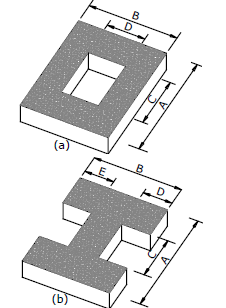
\includegraphics[width=0.15\textwidth]{imagenes/discontinuidades_en_el_sistema_de_piso.png}
\end{figure}

\subsubsection{Ejes estrucutrales no paralelos }
La estructura se considera irregular cuando los ejes estructurales no son paralelos o sim\'etricos 
con respecto a los ejes ortogonales principales de la estructura.

\begin{figure}[h]
    \centering
    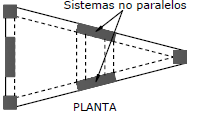
\includegraphics[width=0.15\textwidth]{imagenes/ejes_estructurales_no_paralelos.png}
\end{figure}

\subsection{Irregularidades en elevaci\'on }

\subsubsection{Piso flexible }
La estructura se considera irregular cuando la rigidez lateral de un piso es menor que el 70\% de la rigidez 
lateral del piso superior o menor que el 80 \% del promedio de la rigidez lateral de los tres pisos superiores.
$$K_C < 0.70K_D$$
$$K_C < 0.80 \cdot \dfrac{K_D + K_E + K_F}{3}$$

\begin{figure}[h]
    \centering
    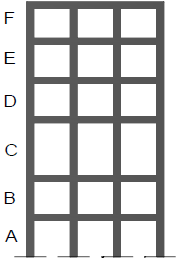
\includegraphics[width=0.15\textwidth]{imagenes/piso_flexible.png}
\end{figure}

\subsubsection{Distribuci\'on de masa }
La estructura se considera irregular cuando la masa de cualquier piso es mayor que 1,5 veces la masa 
de uno de los pisos adyacentes, con excepci\'on del piso de cubierta que sea m\'as liviano que el piso inferior.
$$m_D = 1.50m_E \text{ \'o } m _D > 1.50 m_C$$

\begin{figure}[h]
    \centering
    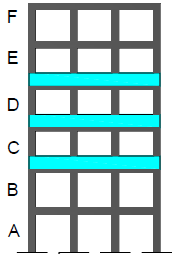
\includegraphics[width=0.15\textwidth]{imagenes/distribucion_de_masa.png}
\end{figure}

\subsubsection{Irregularidad geom\'etrica }
La estructura se considera irregular cuando la dimensi\'on en planta del sistema resistente en cualquier piso 
es mayor que 1,3 veces la misma dimensi\'on en un piso adyacente, exceptuando el caso de los altillos de un solo piso.
$$a > 1.3b$$

\begin{figure}[h]
    \centering
    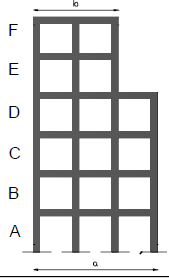
\includegraphics[width=0.15\textwidth]{imagenes/irregularidad_geometrica.png}
\end{figure}

\end{document}